\documentclass[border=4pt]{standalone}

\usepackage{tikz}
\usetikzlibrary{angles, quotes, calc}

\begin{document}
	
	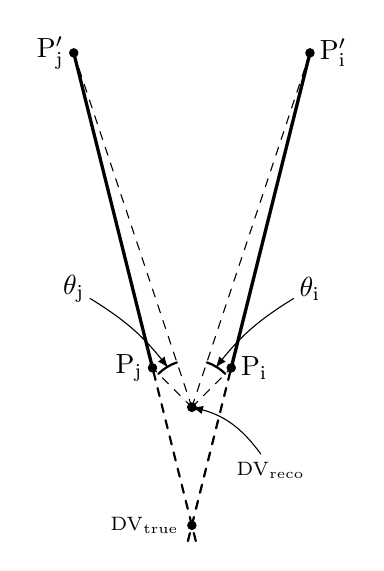
\begin{tikzpicture}[line cap = round]
%		\draw (0,0) grid (10,10);
		
		\coordinate (Ai) at (5,3) {};
		\coordinate (Bi) at (6,7) {};
		\coordinate (Aj) at (4,3) {};
		\coordinate (Bj) at (3,7) {};
		\coordinate (P) at (4.5,2.5) {};
		\node[inner sep = 0.2cm] (DVreco) at ($(P)+(1,-0.8)$) {};
		\coordinate (P') at (4.5,1) {};
		\node[inner sep = 0.2cm] (DVtrue) at ($(P')+(-0.6,0)$) {};
		\node[inner sep = 0.2cm] (thetai) at (6,4) {};
		\node[inner sep = 0.2cm] (thetaj) at (3,4) {};
		
		\draw[very thick] (Ai) -- (Bi);
		\draw[thick, dashed] ($(Ai)!-0.55!(Bi)$) -- (Ai);
		\draw[very thick] (Aj) -- (Bj);
		\draw[thick, dashed] ($(Aj)!-0.55!(Bj)$) -- (Aj);
		\draw[dashed] (P) -- (Ai);
		\draw[dashed] (P) -- (Bi);
		\draw[dashed] (P) -- (Aj);
		\draw[dashed] (P) -- (Bj);
		
		\draw[fill=black] (Ai) circle (1.5pt);
		\draw[fill=black] (Bi) circle (1.5pt);
		\draw[fill=black] (Aj) circle (1.5pt);
		\draw[fill=black] (Bj) circle (1.5pt);
		\draw[fill=black] (P) circle (1.5pt);
		\draw[fill=black] (P) circle (1.5pt);
		\draw[fill=black] (P') circle (1.5pt);
		
		\pic[draw, thick, angle eccentricity=1.4, angle radius=0.6cm] {angle = Ai--P--Bi};
		\pic[draw, thick, angle eccentricity=1.4, angle radius=0.6cm] {angle = Bj--P--Aj};
		
		\node[right] at (Ai) {$\mathrm{P_i}$};
		\node[right] at (Bi) {$\mathrm{P'_i}$};
		\node[left] at (Aj) {$\mathrm{P_j}$};
		\node[left] at (Bj) {$\mathrm{P'_j}$};
		\node at (DVreco) {\scriptsize$\mathrm{DV}_\mathrm{reco}$};
		\node at (DVtrue) {\scriptsize$\mathrm{DV}_\mathrm{true}$};
		\node[] at (thetai) {$\theta_\mathrm{i}$};
		\node[] at (thetaj) {$\theta_\mathrm{j}$};
		
		\draw[-latex] (DVreco) to[bend right=20](P);
		\draw[-latex] (thetai) to[bend right=10](4.8,3);
		\draw[-latex] (thetaj) to[bend left=10](4.2,3);
	\end{tikzpicture}
	
\end{document}